%%%%%%%%%%%%%%%%%%%%%%%%%%%%%%%%%%%%%%%%%%%%%%%%%%%%%%%%%%%%
% INICIO DEL CAPÍTULO 5
%%%%%%%%%%%%%%%%%%%%%%%%%%%%%%%%%%%%%%%%%%%%%%%%%%%%%%%%%%%%

\chapter{Evaluación y Resultados}
\label{chap:implementacion}
Este capítulo presenta la evaluación empírica y los resultados obtenidos al aplicar la metodología propuesta en esta tesis. Para validar la eficacia de la inteligencia artificial como herramienta de análisis de seguridad, la evaluación se desarrolla en dos fases principales.


Primero, se lleva a cabo una rigurosa comparativa entre cuatro modelos de IA de última generación y dos herramientas de referencia en la industria, SonarQube y Snyk. Utilizando un microservicio deliberadamente instrumentado con 13 vulnerabilidades comunes, se mide no solo la capacidad de detección de cada herramienta, sino también aspectos cualitativos como la calidad de las sugerencias de corrección y la profundidad del análisis. Además, se realiza un estudio cuantitativo del rendimiento y el coste computacional, factores cruciales para la viabilidad en un entorno de desarrollo real.


En la segunda parte, se exponen los resultados de la implementación práctica del modelo de IA más equilibrado en un pipeline de Integración y Despliegue Continuo (CI/CD) completamente automatizado. Se demuestra el ciclo completo de detección, bloqueo de código inseguro mediante un \textit{Quality Gate}, facilitación de la remediación a través de reportes accionables y, finalmente, la validación de las correcciones con una ejecución exitosa del pipeline.

\section{Evaluación}
\label{sec:evaluacion}
Para evaluar la eficacia de la integración de la inteligencia artificial en la detección de vulnerabilidades y mejora de la calidad del código, se ha utilizado un microservicio de ejemplo en Java (alojado en el repositorio \url{https://github.com/iJonnathan/TFM/tree/main/demo}), diseñado a propósito con múltiples fallos de seguridad. Este código fue analizado tanto por los modelos de IA como por dos herramientas de referencia que representan el estándar industrial: SonarQube y Snyk.

\subsection{Entorno de Pruebas y Análisis de Vulnerabilidades}

El componente central para la evaluación es el controlador \texttt{WelcomeController.java} y el fichero \texttt{pom.xml} del proyecto, que contienen un conjunto de vulnerabilidades clásicas para medir la capacidad de detección de las herramientas.

\subsubsection{Análisis Detallado de Vulnerabilidades Introducidas}

Para realizar una evaluación controlada, el microservicio de prueba fue deliberadamente instrumentado con un conjunto de vulnerabilidades, representativas de las categorías más comunes del OWASP Top 10. A continuación, se detalla cada una de ellas:

\textbf{1. Clave Secreta Embebida en el Código (CWE-798):} Se han incluido credenciales directamente en el código fuente.
\begin{lstlisting}[language=java, caption={Claves secretas hardcodeadas.}]
// Hardcoded secret (clave embebida)
private static final String DB_PASSWORD = "SuperSecreta123!";
private static final String API_KEY = "ABC123-TOKEN-INSEGURO";
\end{lstlisting}

\textbf{2. Cross-Site Scripting (XSS) Reflejado (CWE-79):} El endpoint \texttt{/api/welcome} concatena un parámetro en la respuesta sin saneamiento.
\begin{lstlisting}[language=java, caption={Código vulnerable a XSS.}]
@GetMapping("/api/welcome")
public WelcomeDTO welcome( @RequestParam(value = "name", defaultValue = "...") String name) {
    return new WelcomeDTO("Hola, bienvenido " + name + ", esto es un demo");
}
\end{lstlisting}

\textbf{3. Ejecución Remota de Código (RCE) (CWE-94):} El endpoint \texttt{/api/execute} evalúa una cadena del usuario como código, permitiendo la ejecución de comandos arbitrarios.
\begin{lstlisting}[language=java, caption={Código vulnerable a RCE.}]
@PostMapping("/api/execute")
public String executeCode( @RequestBody String userScript) throws Exception {
    ScriptEngine engine = new ScriptEngineManager().getEngineByName("nashorn");
    return "Resultado: " + engine.eval(userScript);
}
\end{lstlisting}

\textbf{4. Path Traversal (CWE-22):} El endpoint \texttt{/api/read-file} permite leer archivos del sistema sin una validación de ruta adecuada.
\begin{lstlisting}[language=java, caption={Código vulnerable a Path Traversal.}]
@GetMapping("/api/read-file")
public String readFile( @RequestParam String filePath) throws Exception {
    return Files.readString(Paths.get(filePath));
}
\end{lstlisting}

\textbf{5. Inyección SQL (CWE-89):} El endpoint \texttt{/api/user} construye una consulta SQL concatenando directamente la entrada del usuario.
\begin{lstlisting}[language=java, caption={Código vulnerable a Inyección SQL.}]
@GetMapping("/api/user")
public String getUserInfo( @RequestParam String username) throws Exception {
    Connection conn = DriverManager.getConnection("jdbc:mysql://localhost:3306/demo", "root", DB_PASSWORD);
    Statement stmt = conn.createStatement();
    ResultSet rs = stmt.executeQuery("SELECT * FROM users WHERE username = '" + username + "'");
    // ...
}
\end{lstlisting}

\textbf{6. Inyección de Comandos (CWE-78):} El endpoint \texttt{/api/ping} ejecuta un comando del sistema operativo concatenando la entrada del usuario.
\begin{lstlisting}[language=java, caption={Código vulnerable a Inyección de Comandos.}]
@PostMapping("/api/ping")
public String ping( @RequestBody String host) throws Exception {
    Process p = Runtime.getRuntime().exec("ping -c 1 " + host);
    // ...
}
\end{lstlisting}

\textbf{7. Deserialización Insegura (CWE-502):} El endpoint \texttt{/api/deserialize} deserializa un objeto de una fuente no confiable sin validación.
\begin{lstlisting}[language=java, caption={Código vulnerable a Deserialización Insegura.}]
@PostMapping("/api/deserialize")
public String deserialize( @RequestBody String base64) throws Exception {
    byte[] data = Base64.getDecoder().decode(base64);
    ObjectInputStream ois = new ObjectInputStream(new ByteArrayInputStream(data));
    Object obj = ois.readObject();
    return "Objeto: " + obj;
}
\end{lstlisting}

\textbf{8. Inserción de Información Sensible en Logs (CWE-532):} El endpoint \texttt{/api/login} registra credenciales en texto plano.
\begin{lstlisting}[language=java, caption={Logs con información sensible.}]
@PostMapping("/api/login")
public String login( @RequestParam String user, @RequestParam String password) {
    logger.info("Intento de login con usuario: " + user + " y contraseña: " + password); // Log inseguro
    return "Login procesado";
}
\end{lstlisting}

\textbf{9. Uso de Criptografía Débil (CWE-327):} El endpoint \texttt{/api/hash} utiliza el algoritmo MD5, que está criptográficamente roto.
\begin{lstlisting}[language=java, caption={Uso de un algoritmo de hash débil (MD5).}]
@GetMapping("/api/hash")
public String hash( @RequestParam String data) throws Exception {
    MessageDigest md = MessageDigest.getInstance("MD5"); // Inseguro
    byte[] digest = md.digest(data.getBytes());
    return Base64.getEncoder().encodeToString(digest);
}
\end{lstlisting}

\textbf{10. Cifrado Simétrico Débil (CWE-326):} El endpoint \texttt{/api/encrypt} usa AES con una clave estática y sin un modo de operación seguro (como GCM).
\begin{lstlisting}[language=java, caption={Cifrado simétrico débil (AES con clave fija).}]
@GetMapping("/api/encrypt")
public String encrypt( @RequestParam String text) throws Exception {
    String key = "1234567890123456"; // Clave estática
    SecretKeySpec secretKey = new SecretKeySpec(key.getBytes(), "AES");
    Cipher cipher = Cipher.getInstance("AES"); // sin GCM ni IV
    cipher.init(Cipher.ENCRYPT_MODE, secretKey);
    return Base64.getEncoder().encodeToString(cipher.doFinal(text.getBytes()));
}
\end{lstlisting}

\textbf{11. Exposición de Información Sensible por Error (CWE-209):} El endpoint \texttt{/api/error} devuelve detalles de la excepción al usuario.
\begin{lstlisting}[language=java, caption={Manejo de excepciones que expone información.}]
@GetMapping("/api/error")
public String error() {
    try {
        int a = 1 / 0;
        return "OK";
    } catch (Exception e) {
        return e.toString(); // Devuelve detalles internos
    }
}
\end{lstlisting}

\textbf{12. Dependencia Vulnerable (CWE-1104):} Se incluyó una versión antigua de la librería `jackson-databind` en el `pom.xml`, conocida por tener vulnerabilidades de deserialización.
\begin{lstlisting}[language=xml, caption={Dependencia vulnerable en pom.xml.}]
<dependency>
    <groupId>com.fasterxml.jackson.core</groupId>
    <artifactId>jackson-databind</artifactId>
    <version>2.9.8</version> 
</dependency>
\end{lstlisting}

\subsection{Modelos y Herramientas de Análisis}

Para llevar a cabo una evaluación exhaustiva y comparativa, se seleccionó un conjunto de modelos de IA de vanguardia y dos herramientas de referencia líderes en la industria.

Los modelos de IA, todos accesibles a través de la plataforma OpenRouter, fueron:
\begin{itemize}
    \item \textbf{google/gemini-2.0-flash-exp:free}: Un modelo de última generación de Google, conocido por su velocidad y capacidades multimodales.
    \item \textbf{deepseek/deepseek-chat:free}: Un modelo de DeepSeek AI especializado y afinado para tareas de conversación y codificación.
    \item \textbf{deepseek/deepseek-r1-0528:free}: Un modelo de código abierto de DeepSeek de alto rendimiento.
    \item \textbf{qwen/qwen-2.5-coder-32b-instruct:free}: Un modelo de Qwen (Alibaba) especializado en código.
\end{itemize}

\paragraph{Herramientas de Referencia (Baselines).}
\begin{itemize}
\item \textbf{SonarQube Community Edition 9.9}: Representa la línea base para el Análisis Estático de Seguridad de
Aplicaciones (SAST) y la calidad del código. Es una de las herramientas más utilizadas en la industria para el análisis del código fuente propio.
\item \textbf{Snyk Open Source}: Representa la línea base para el Análisis de Composición de Software (SCA). Se utilizó la funcionalidad disponible en su plan gratuito, que se enfoca en detectar vulnerabilidades en dependencias de terceros. Es pertinente mencionar que Snyk también ofrece una solución SAST comercial (\textit{Snyk Code}), pero sus capacidades completas forman parte de sus planes de pago y no fueron objeto de esta evaluación \cite{snyk_plans}.
\end{itemize}

\subsection{Análisis Comparativo de Resultados}
\label{subsec:analisis_comparativo_resultados}
Cada modelo de IA y las herramientas de referencia analizaron el proyecto. La siguiente tabla detalla la detección de cada vulnerabilidad específica.

\newcommand{\cmark}{{\color{green!80!black}\checkmark}}%
\newcommand{\xmark}{{\color{red!80!black}\ding{55}}}%

\begin{table}[H]
\centering
\caption{Detección Detallada de Vulnerabilidades por Herramienta}
\label{tab:comparativa_detallada}
\resizebox{\textwidth}{!}{%
\begin{tabular}{|l|c|c|c|c|c|c|}
\hline
\textbf{Vulnerabilidad} & \textbf{SonarQube} & \textbf{Snyk (Free)} & \textbf{Gemini 2.0} & \textbf{DS Chat} & \textbf{DS R1} & 
\textbf{Qwen 2.5} \\
\hline
Hardcoded Secret (Password) & \cmark & N/A & \cmark & \cmark & \cmark & \cmark \\
\hline
Hardcoded Secret (API Key) & \cmark & N/A & \cmark & \cmark & \cmark & \cmark \\
\hline
Cross-Site Scripting (XSS) & \xmark & N/A & \cmark & \cmark & \cmark & \cmark \\
\hline
Remote Code Execution (RCE) & \xmark & N/A & \cmark & \cmark & \cmark & \cmark \\
\hline
Path Traversal & \xmark & N/A & \cmark & \cmark & \cmark & \cmark \\
\hline
Inyección SQL (SQLi) & \xmark & N/A & \cmark & \cmark & \cmark & \cmark \\
\hline
Inyección de Comandos & \xmark & N/A & \cmark & \cmark & \cmark & \cmark \\
\hline
Deserialización Insegura & \xmark & N/A & \cmark & \cmark & \cmark & \cmark \\
\hline
Logs con Datos Sensibles & \xmark & N/A & \cmark & \cmark & \cmark & \cmark \\
\hline
Uso de Criptografía Débil (Hash) & \xmark & N/A & \cmark & \cmark & \cmark & \cmark \\
\hline
Cifrado Simétrico Débil & \cmark & N/A & \cmark & \cmark & \cmark & \cmark \\
\hline
Exposición de Error (Stacktrace) & \xmark & N/A & \cmark & \cmark & \cmark & \cmark \\
\hline
Dependencia Vulnerable (pom.xml) & \xmark & \cmark & \cmark & \cmark & \cmark & \cmark \\
\hline
\hline
\textbf{Total Código Fuente (12)} & 3 & N/A & 12 & 12 & 12 & 12 \\
\hline
\textbf{Total Dependencias (1)} & 0 & 1 & 1 & 1 & 1 & 1 \\
\hline
\end{tabular}%
}
\end{table}

\subsubsection{Análisis Cualitativo de las Respuestas de IA}

Como se estableció en la tabla \ref{tab:comparativa_detallada}, todos los modelos de IA demostraron una capacidad de detección del 100\% en el entorno de prueba. Este resultado, aunque impresionante, oculta diferencias cualitativas importantes en las respuestas que son críticas para un entorno de desarrollo real. A continuación, se analizan ejemplos concretos que ilustran estas diferencias.

\paragraph{Profundidad y Seguridad de la Sugerencia de Corrección.}
Un buen indicador de la calidad de un modelo es la robustez de la solución que propone. Se puede observar una diferencia clara en la gestión de la vulnerabilidad de \textbf{Path Traversal (CWE-22)}.


\begin{itemize}
    \item El modelo \textbf{qwen/qwen-2.5-coder-32b-instruct:free} ofreció la siguiente sugerencia:
    \begin{lstlisting}[language=java,caption={Sugerencia de Qwen para Path Traversal.}]
// Sugerencia de corrección:
if (!filePath.startsWith("/safe/directory/")) {
    throw new IllegalArgumentException("Ruta inválida");
}
    \end{lstlisting}
    \textbf{Análisis:} Esta solución es superficial e insegura. Un atacante podría evadirla fácilmente utilizando secuencias de escape como `filePath = ``/safe/directory/../../etc/passwd'' ', ya que la cadena efectivamente comienza con el prefijo permitido, pero luego navega fuera del directorio seguro.

    \item En contraste, los modelos \textbf{google/gemini-2.0-flash-exp:free} y \textbf{deepseek/deepseek-r1-0528:free} proporcionaron una solución mucho más robusta y segura:
    \begin{lstlisting}[language=java,caption={Sugerencia de Gemini/DeepSeek para Path Traversal.}]
// Sugerencia de corrección:
Path safePath = Paths.get("/safe/directory/").resolve(filePath).normalize();
if (!safePath.startsWith(Paths.get("/safe/directory/"))) {
    throw new IllegalArgumentException("Invalid file path");
}
return Files.readString(safePath);
    \end{lstlisting}
    \textbf{Análisis:} Esta implementación es significativamente superior. El método `.normalize()` resuelve las secuencias `..`, eliminando los intentos de evasión. La posterior validación con `.startsWith()` sobre la ruta ya normalizada asegura que el acceso a ficheros se mantenga estrictamente dentro del directorio previsto. Este es un ejemplo claro de cómo, a pesar de que ambos modelos detectaron la vulnerabilidad, solo uno proporcionó una corrección verdaderamente segura y accionable para el desarrollador.
\end{itemize}

\paragraph{Riqueza del Análisis: Más Allá de la Seguridad.}
Otro diferenciador clave es la capacidad de algunos modelos para ofrecer observaciones valiosas sobre la calidad y mantenibilidad del código, incluso en ficheros sin vulnerabilidades de seguridad. El análisis del fichero \texttt{WelcomeDTO.java} (un simple DTO) es un buen ejemplo.

\begin{itemize}
    \item El modelo \textbf{deepseek/deepseek-r1-0528:free} identificó una mejora de fiabilidad importante:
    \begin{quote}
        \textbf{Descripción:} Class does not override equals() and hashCode(). This may cause unexpected behavior when used in collections. \\
        \textbf{Recomendación:} Implement equals() and hashCode() based on the message field.
    \end{quote}
    \textbf{Análisis:} Esta es una sugerencia de alta calidad. No implementar `equals()` y `hashCode()` en DTOs es una causa frecuente de comportamientos anómalos y errores de difícil depuración cuando estos objetos se utilizan en colecciones como `HashMap` o `HashSet`. Este tipo de feedback proactivo ayuda a mejorar la robustez general de la aplicación.

    \item Por su parte, el modelo \textbf{google/gemini-2.0-flash-exp:free} se enfocó en un principio de diseño de software:
    \begin{quote}
        \textbf{Descripción:} The `message` field is mutable due to the presence of a setter method. For simple DTOs, immutability can improve thread safety and predictability. \\
        \textbf{Recomendación:} If the message should not be changed after creation, remove the `setMessage` method and make the `message` field final.
    \end{quote}
    \textbf{Análisis:} Esta también es una recomendación valiosa que apunta a mejorar la mantenibilidad y a prevenir efectos secundarios no deseados, promoviendo un diseño más funcional y seguro en entornos concurrentes.
\end{itemize}

Estos ejemplos demuestran que, si bien la cobertura de detección de vulnerabilidades es una métrica base, la verdadera diferenciación y el valor para un equipo de desarrollo radican en la calidad, profundidad y seguridad de las recomendaciones generadas, así como en la capacidad del modelo para actuar como un revisor de código integral.

\subsubsection{Análisis Cuantitativo de Rendimiento y Coste}

Más allá de la calidad de la detección, la viabilidad de integrar una solución de IA en un pipeline de CI/CD depende críticamente de dos factores cuantitativos: el \textbf{rendimiento} (tiempo de ejecución) y el \textbf{coste} (consumo de tokens). Un análisis lento puede crear cuellos de botella en el ciclo de desarrollo, mientras que un alto consumo de tokens puede hacer que la solución sea económicamente inviable a escala.

\paragraph{La Importancia de los Tokens.} En los modelos de IA comerciales, el coste se factura por el número de \textit{tokens} procesados. Un token es una unidad de texto (aproximadamente 4 caracteres en inglés). El coste total de una llamada a la API se compone de:
\begin{itemize}
    \item \textbf{Tokens de Entrada (Prompt Tokens):} El tamaño del código y las instrucciones enviadas al modelo. En este experimento, los tokens de entrada fueron constantes para todos los modelos, ya que analizaron los mismos ficheros.
    \item \textbf{Tokens de Salida (Completion Tokens):} El tamaño de la respuesta JSON generada por el modelo. Una respuesta más detallada, con descripciones más largas y sugerencias de código más elaboradas, consume más tokens de salida y, por lo tanto, es más costosa.
\end{itemize}

Para evaluar estos factores, se midió el tiempo de ejecución de cada análisis y se utilizó el tamaño en bytes del fichero de resultados JSON como una métrica proxy del consumo de tokens de salida.
\begin{table}[H]
    \centering
    \caption{Comparativa de Rendimiento y Consumo de Tokens}
    \label{tab:rendimiento_coste}
    \begin{tabular}{|l|c|c|l|}
        \hline
        \textbf{Modelo de IA}                   & \textbf{\makecell{Tiempo de \\ Análisis}} & \textbf{\makecell{Tamaño de \\ Respuesta \\ (Proxy de Tokens)}} & \textbf{Análisis} \\
        \hline
        gemini-2.0-flash-exp:free           & 1 min 38 seg                              & 45.6 KB                                                         & Rápido y detallado \\
        \hline
        deepseek-chat:free                  & 8 min 13 seg                              & 24.8 KB                                                         & \makecell[l]{Lento y moderadamente \\ detallado} \\
        \hline
        deepseek-r1-0528:free               & 18 min 49 seg                             & 16.1 KB                                                         & Muy lento y conciso \\
        \hline
        qwen-2.5-coder-32b-instruct:free    & 4 min 54 seg                              & 49.2 KB                                                & \makecell[l]{Velocidad media, \\ respuesta más extensa} \\
        \hline
    \end{tabular}
\end{table}

\paragraph{Discusión de los Resultados.}
La Tabla \ref{tab:rendimiento_coste} revela un interesante equilibrio entre velocidad, coste y verbosidad:
\begin{itemize}
    \item El modelo \textbf{qwen/qwen-2.5-coder-32b-instruct:free} generó la respuesta más detallada (mayor tamaño), lo que implica un mayor coste en tokens, pero lo hizo en un tiempo razonable. Esto sugiere que es un modelo que prioriza la exhaustividad en sus explicaciones.
    \item El modelo \textbf{google/gemini-2.0-flash-exp:free} emerge como el más equilibrado para un entorno de CI/CD. Ofrece una velocidad de ejecución excepcional (casi 5 veces más rápido que el siguiente) y genera una respuesta muy detallada, representando una excelente relación entre eficiencia, coste y calidad de la información.
    \item El modelo \textbf{deepseek/deepseek-r1-0528:free}, a pesar de ser el más lento, fue sorprendentemente el más conciso en su respuesta. Esto indica un estilo de comunicación muy directo, que podría ser preferible en algunos contextos, pero su alto tiempo de ejecución lo hace menos ideal para pipelines de integración continua que requieren retroalimentación rápida.
\end{itemize}

Este análisis cuantitativo es fundamental para la toma de decisiones en un entorno real. Un equipo podría optar por usar un modelo rápido y económico como \texttt{google/gemini-2.0-flash-exp:free} para las revisiones en cada commit, y reservar el uso de un modelo más lento pero potencialmente más exhaustivo en sus explicaciones para los escaneos nocturnos o previos al despliegue.


Del análisis detallado de los resultados, se extraen las siguientes observaciones clave:

\begin{itemize}
    \item \textbf{Rendimiento de las Herramientas de Referencia (Baselines)}: Las herramientas especializadas demostraron ser eficaces en sus respectivos dominios, pero limitadas fuera de ellos.
        \begin{itemize}
            \item \textbf{SonarQube (SAST)}: Detectó 3 de las 12 vulnerabilidades presentes en el código fuente, enfocándose en patrones evidentes como las claves embebidas. Sin embargo, no identificó ninguna vulnerabilidad contextual (SQLi, XSS) ni la dependencia vulnerable en el \texttt{pom.xml}.
            \item \textbf{Snyk (SCA)}: Como se esperaba de una herramienta SCA líder, identificó con éxito la dependencia vulnerable en el el \texttt{pom.xml} (`jackson-databind`), proporcionando un listado exhaustivo de los 58 problemas de seguridad asociados a esa única dependencia. No obstante, su alcance no cubre el análisis del código fuente propio.
        \end{itemize}

    \item \textbf{Rendimiento Holístico de los Modelos de IA}: El hallazgo más significativo es la capacidad de los modelos de IA para realizar un análisis híbrido, cubriendo tanto las responsabilidades de SAST como de SCA con una eficacia del 100\% en el entorno de prueba. Todos los modelos identificaron la totalidad de las 13 vulnerabilidades, demostrando una comprensión contextual del código y una capacidad para analizar las dependencias del proyecto. Esto representa una ventaja fundamental, ya que ofrecen una visión de seguridad unificada que tradicionalmente requeriría la integración de múltiples herramientas especializadas.

    \item \textbf{Nuevos Criterios de Diferenciación}: Dado que todos los modelos de IA alcanzaron la máxima puntuación en detección, la diferenciación entre ellos ya no se basa en la cobertura, sino en otros factores cualitativos y cuantitativos:
        \begin{itemize}
            \item \textbf{Velocidad y Coste}: Como se observó previamente, existe un claro compromiso. Modelos como google/gemini-2.0-flash-exp:free ofrecen resultados casi instantáneos, mientras que otros como deepseek/deepseek-r1-0528:free son más lentos, lo que puede influir en la elección para distintos tipos de pipelines (CI vs. CD).
            \item \textbf{Calidad del Reporte}: Aunque todos detectaron las vulnerabilidades, la calidad y claridad de las descripciones y, sobre todo, de las sugerencias de corrección, varía entre modelos. Este factor cualitativo es crucial para la accionabilidad de los resultados por parte de los desarrolladores.
            \item \textbf{Análisis de Calidad de Código}: Además de la seguridad, modelos como deepseek-r1-0528:free también proporcionaron un análisis más rico sobre la calidad general del código, similar al de SonarQube, aportando un valor añadido.
        \end{itemize}

    \item \textbf{Complementariedad Re-evaluada}: La idea de complementariedad sigue siendo válida, pero con un nuevo matiz. SonarQube es fundamental para aplicar un conjunto de reglas de código de forma rápida y consistente. La IA, por su parte, no solo complementa, sino que asume el rol principal en la detección de vulnerabilidades de seguridad, ofreciendo una cobertura que antes solo era posible con herramientas comerciales muy costosas o revisiones manuales exhaustivas.
\end{itemize}

\subsection{Conclusión de la Evaluación}

La evaluación empírica llevada a cabo en este trabajo permite extraer una conclusión fundamental: la integración de la Inteligencia Artificial en los pipelines de CI/CD para el análisis de seguridad no solo es una propuesta viable, sino que supera de manera significativa la capacidad de las herramientas de análisis estático gratuitas, como SonarQube Community Edition, en la detección de vulnerabilidades de seguridad complejas.

Mientras que SonarQube se mantiene como una herramienta indispensable para gobernar y mantener la calidad, la fiabilidad y la mantenibilidad del código base, los modelos de IA evaluados han demostrado llenar un vacío crítico en la estrategia de DevSecOps. Su capacidad para realizar un análisis semántico y contextual del código les permite identificar riesgos de seguridad de alto impacto que a menudo pasan desapercibidos para los analizadores basados en reglas estáticas.

La elección final de la herramienta o modelo a integrar dependerá de los objetivos específicos y las restricciones del pipeline de cada organización:
\begin{itemize}
    \item \textbf{Para Calidad de Código y Mantenibilidad}: SonarQube Community sigue siendo la herramienta de referencia indiscutible.
    \item \textbf{Para Máxima Precisión y Cobertura en Seguridad}: El modelo deepseek-r1-0528 demostró ser la opción más segura y exhaustiva, ideal para ejecuciones en pipelines de despliegue a producción o en escaneos de seguridad programados y profundos donde la cobertura total es el objetivo principal.
    \item \textbf{Para un Balance Óptimo entre Seguridad y Agilidad en CI/CD}: Los modelos gemini-2.0-flash-exp y deepseek-chat ofrecen un excelente compromiso, detectando la gran mayoría de las vulnerabilidades críticas en un tiempo de ejecución que se adapta bien a un pipeline de desarrollo activo.
\end{itemize}

En definitiva, una estrategia de DevSecOps madura debería considerar un enfoque híbrido, utilizando SonarQube para establecer una base sólida de calidad de código y complementándolo con un modelo de IA para realizar un análisis de seguridad contextual y profundo, automatizando así una defensa en profundidad directamente en el ciclo de vida del desarrollo.

%%%%%%%%%%%%%%%%%%%%%%%%%%%%%%%%%%%%%%%%%%%%%%%%%%%%%%%%%%%%%%%%%%%%%%%
% FIN DEL CAPÍTULO 4
%%%%%%%%%%%%%%%%%%%%%%%%%%%%%%%%%%%%%%%%%%%%%%%%%%%%%%%%%%%%%%%%%%%%%%%
\section{Resultados de la Ejecución del Pipeline}
\label{subsec:analisis_resultados_pipeline}

Para la validación empírica de la solución, se seleccionó el modelo de IA gemini-2.0-flash-exp. Esta elección se basa en los resultados obtenidos en la evaluación comparativa de modelos detallada en la sección \ref{subsec:analisis_comparativo_resultados}, el cual evidenció el mejor equilibrio entre precisión, calidad de las sugerencias y eficiencia.

Con el entorno CI/CD completamente automatizado, se procedió a ejecutar el pipeline para el microservicio de prueba (`demo`). La ejecución se activó tras un `commit` en el repositorio, demostrando el cumplimiento del requisito \textbf{RF-01}. La vista general de la ejecución del pipeline, mostrando las etapas completadas y el punto de fallo, se puede apreciar en la Figura \ref{fig:pipeline_general_fail}.

\begin{figure}[h]
\centering
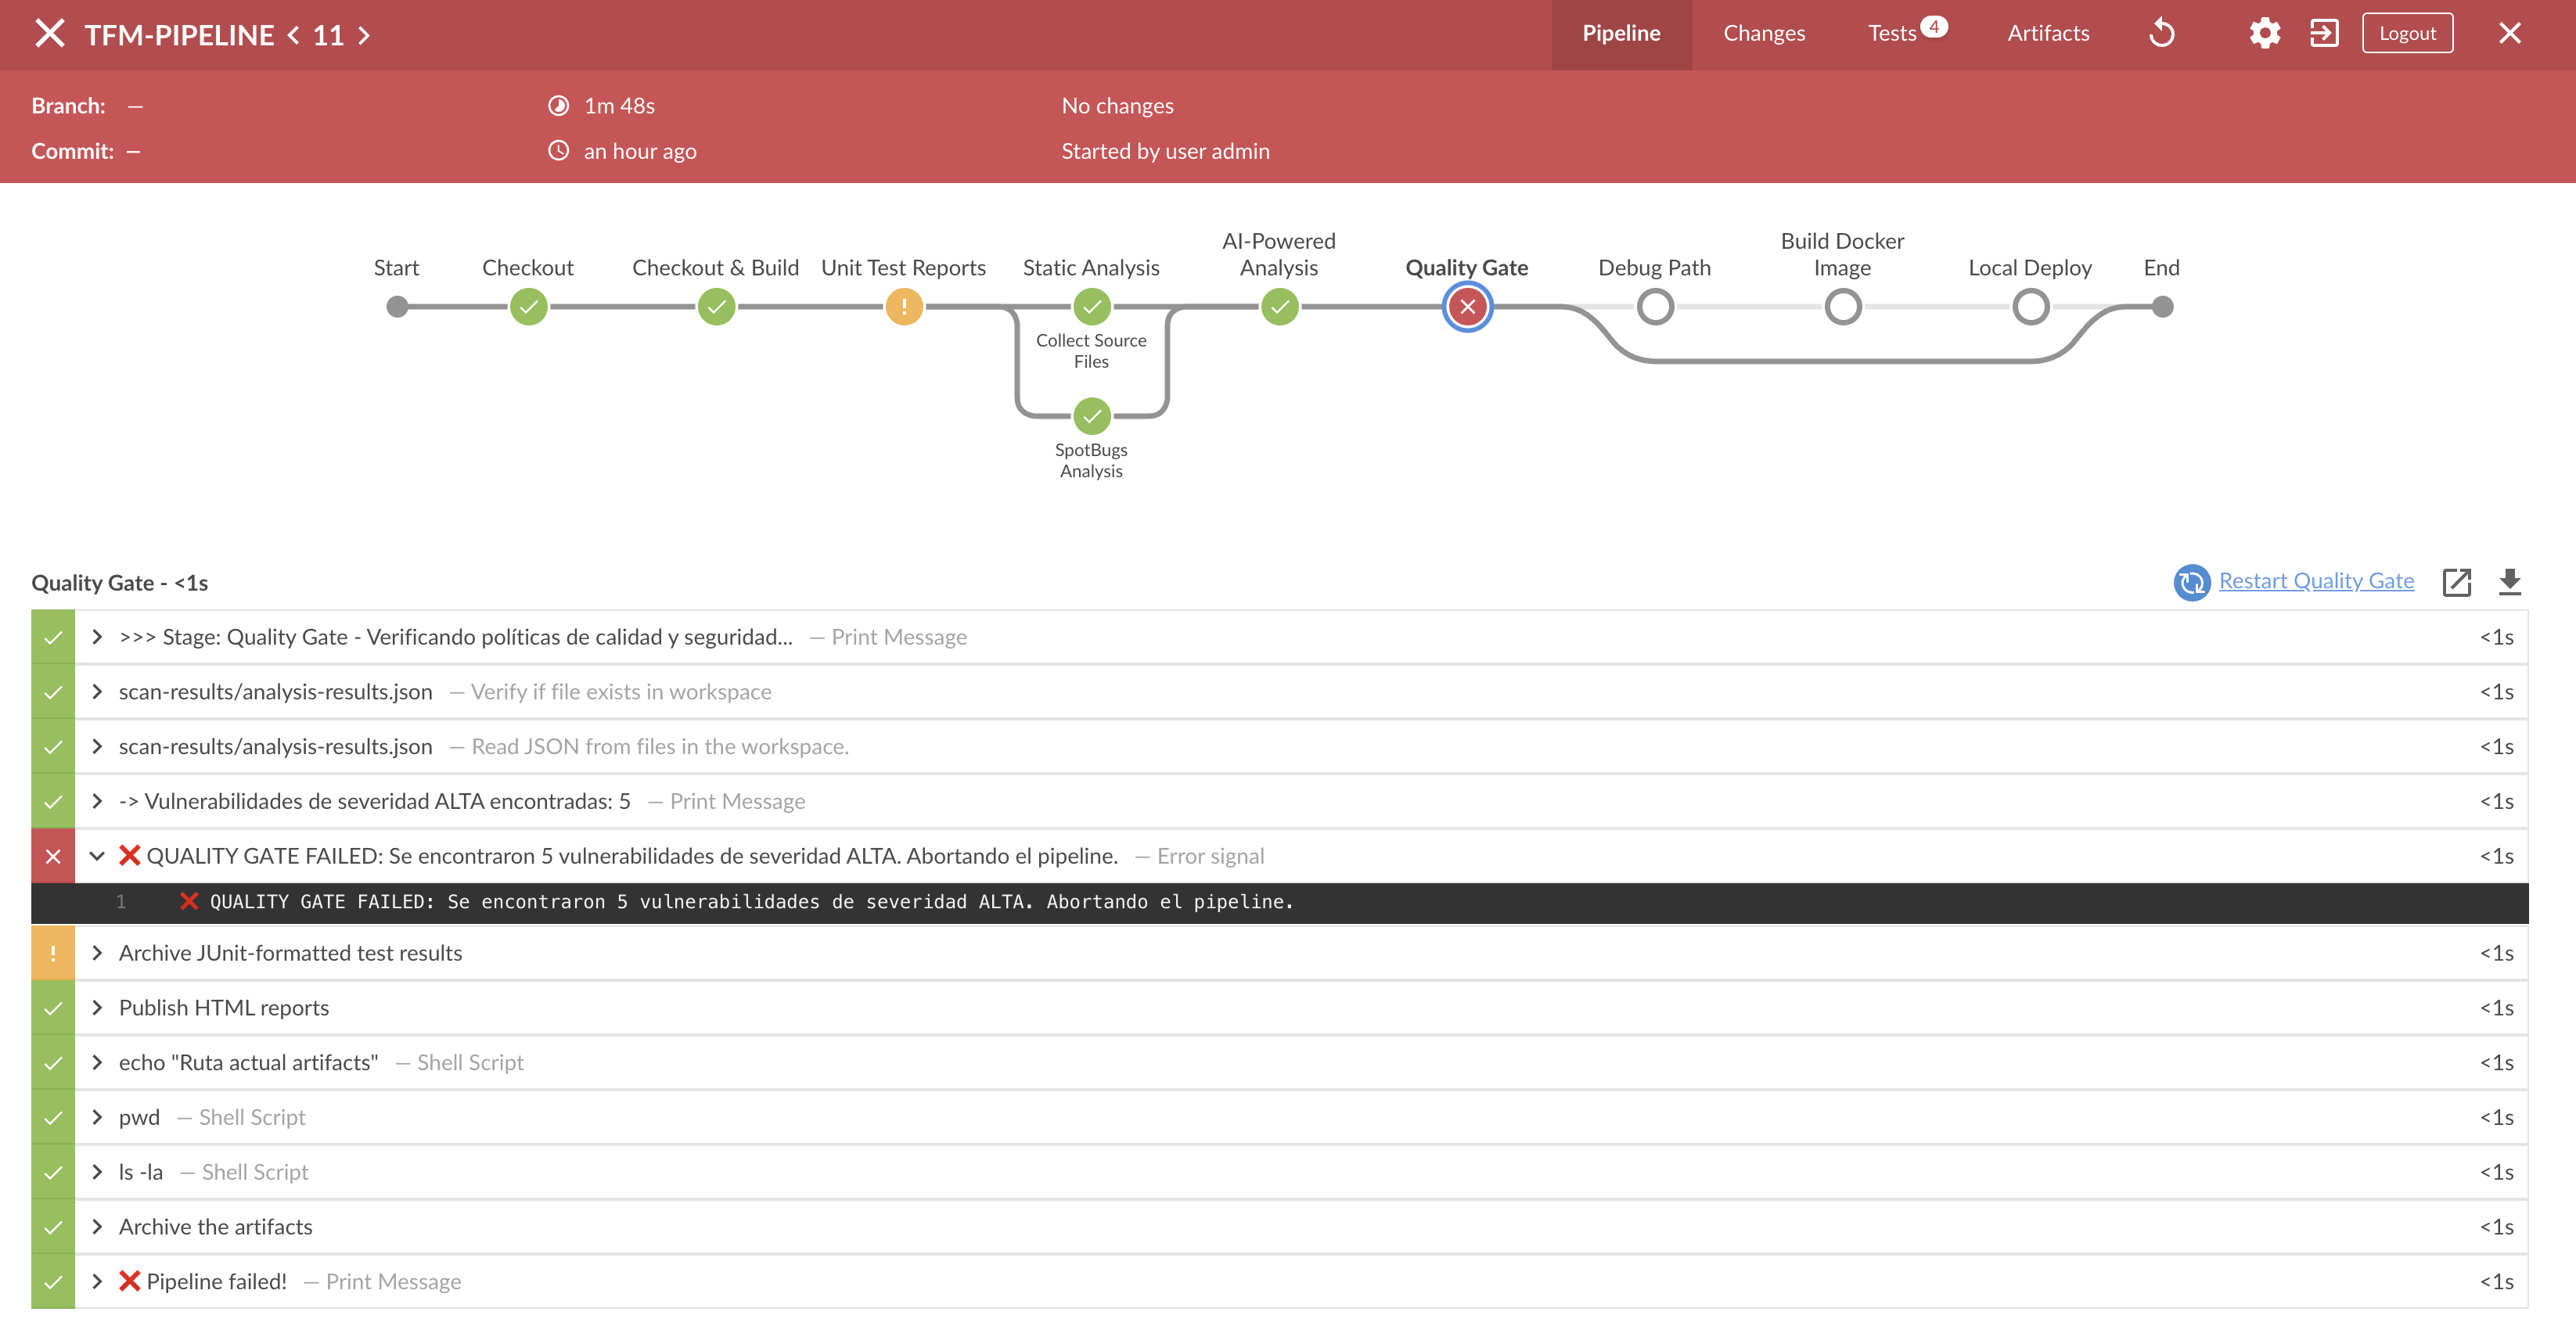
\includegraphics[width=0.99\textwidth]{contenido/imagenes/4_pipeline_fail.png}
\caption{Ejecución fallida del pipeline.}
\label{fig:pipeline_general_fail}
\end{figure}

\subsubsection{Flujo de Ejecución y Falla Controlada en el Quality Gate}
El pipeline ejecutó las primeras etapas de manera secuencial y paralela, tal como fue diseñado, recopilando información de seguridad en cada paso antes de llegar al punto de control crítico.

\begin{enumerate}
    \item Las etapas iniciales, \textbf{Checkout \& Build} y \textbf{Unit Test Reports}, se completaron con éxito. El código fue clonado, la aplicación fue empaquetada con Maven (\textbf{RF-02}), y los reportes de pruebas unitarias fueron procesados por Jenkins, sin embargo, una de las pruebas unitarias saltó una excepción debido a una vulnerabilidad de dependencia en el pom.xml, el cual fue detectada en el stage AI-Powered Analysis.
    \item La etapa \textbf{Static Analysis} se ejecutó, realizando sus tareas en paralelo para optimizar el tiempo.
    \item La etapa \textbf{AI-Powered Analysis} se completó satisfactoriamente, cumpliendo su objetivo principal (\textbf{RF-04}). El script de Python interactuó con la API de la IA y generó los artefactos cruciais: el reporte HTML para el desarrollador (`ai-analysis-report.html`) y el reporte JSON (`analysis-results.json`) para la automatización, cumpliendo así con \textbf{RF-05}.
    \item La ejecución llegó a la etapa \textbf{Quality Gate}. Este es el punto de control automatizado que implementa la política de seguridad del pipeline. El script leyó el archivo analysis-results.json y, tal como se esperaba, encontró que el valor de high\_severity\_vulnerabilities era de 5. 
\end{enumerate}

Debido a que este valor era mayor que el umbral de cero definido en la política, la condición del Quality Gate se activó y ejecutó el paso error(). Este comando detuvo inmediatamente el pipeline y lo marcó con el estado \textbf{FAILURE}, como se evidencia en la captura de la Figura \ref{fig:pipeline_general_fail}. Como resultado, las etapas posteriores Debug Path, Build Docker Image y Local Deploy nunca se ejecutaron.

Este fallo controlado es un éxito rotundo para el experimento. Demuestra que el sistema funciona como un mecanismo de seguridad preventivo eficaz (cumpliendo \textbf{RF-06}), deteniendo físicamente la promoción de código inseguro a través del ciclo de vida de desarrollo.

\subsubsection{Análisis Detallado del Reporte Generado por la IA}
La pieza clave generada por el pipeline es el reporte en formato HTML. Este documento, fácil de leer para los desarrolladores, es la principal herramienta para entender y solucionar los problemas encontrados. El reporte completo de esta ejecución se encuentra en el \textbf{Anexo \ref{anexo:ai-analysis-report}}.

A continuación, se explican los problemas más graves que encontró la IA y que causaron la falla del Quality Gate.

\paragraph{Dependencia Vulnerable en `pom.xml` (Severidad: HIGH)}
\begin{itemize}
    \item \textbf{Hallazgo:} La IA revisó el archivo pom.xml y vio que se usaba la versión 2.9.8 de la librería jackson-databind. Avisó que esta versión es muy antigua y tiene fallos de seguridad graves (CVEs) que podrían permitir a un atacante ejecutar código en el servidor.
    \item \textbf{Sugerencia de la IA:} La solución fue simple y directa: actualizar la librería a una versión más nueva y segura (como 2.16.1 o superior) en el archivo pom.xml.
\end{itemize}

\paragraph{Inyección SQL (Severidad: CRITICAL)}
\begin{itemize}
    \item \textbf{Hallazgo:} En el WelcomeController, la IA detectó que una consulta a la base de datos se estaba construyendo uniendo texto con datos que venían de un usuario, sin ninguna protección. Esto es un riesgo clásico de Inyección SQL.
    \item \textbf{Sugerencia de la IA:} Recomendó usar consultas preparadas (PreparedStatement), que es la forma correcta y segura de hacerlo, e incluyó un ejemplo de código de cómo implementarlo.
\end{itemize}

\paragraph{Ejecución Remota de Código (RCE) (Severidad: CRITICAL)}
\begin{itemize}
    \item \textbf{Hallazgo:} El sistema identificó que una parte del código ScriptEngine.eval() ejecutaba comandos directamente de la entrada del usuario, lo que es un riesgo crítico.
    \item \textbf{Sugerencia de la IA:} La recomendación fue eliminar esa función por completo, lo cual es la decisión más segura cuando una característica es tan peligrosa.
\end{itemize}

\paragraph{Path Traversal (Severidad: HIGH)}
\begin{itemize}
    \item \textbf{Hallazgo:} La IA señaló que una función que leía archivos tomaba la ruta del archivo directamente de la entrada del usuario, lo que le permitiría a un atacante leer archivos prohibidos del sistema usando secuencias como `../`.
    \item \textbf{Sugerencia de la IA:} Sugirió añadir código para verificar que la ruta del archivo solicitado estuviera siempre dentro de una carpeta base segura y permitida.
\end{itemize}

\paragraph{Claves Secretas en el Código (Severidad: CRITICAL)}
\begin{itemize}
    \item \textbf{Hallazgo:} El modelo encontró que la contraseña de la base de datos y una clave de API estaban escritas directamente en el código.
    \item \textbf{Sugerencia de la IA:} Recomendó seguir las mejores prácticas de seguridad (cumpliendo \textbf{RNF-03}) y mover estos secretos a variables de entorno o a un sistema de gestión de credenciales, en lugar de tenerlos en el código.
\end{itemize}
\subsubsection{Remediación y Ejecución Exitosa del Pipeline}
\label{subsec:remediacion_exitosa}

El valor fundamental del prototipo no reside únicamente en la detección, sino en su capacidad para facilitar una remediación rápida y precisa. Con las instrucciones claras y los ejemplos de código proporcionados por el reporte de la IA, un desarrollador pudo proceder a corregir las 5 vulnerabilidades críticas identificadas. El proceso de remediación consistió en:
\begin{itemize}
    \item Actualizar la versión de la dependencia `jackson-databind` en el archivo `pom.xml` a una versión segura.
    \item Refactorizar el método `getUserInfo` en WelcomeController.java para utilizar PreparedStatement, eliminando así la vulnerabilidad de Inyección SQL.
    \item Eliminar por completo los métodos inseguros executeCode (RCE) y ping (Command Injection).
    \item Añadir la lógica de validación de rutas en el método readFile para prevenir el Path Traversal.
    \item Externalizar las claves secretas (`DB\_PASSWORD` y `API\_KEY`), eliminándolas del código fuente y configurándolas como variables de entorno seguras.
\end{itemize}

Una vez aplicados estos cambios y subido el código corregido al repositorio de GitHub, el pipeline de Jenkins se ejecutó por segunda vez.

En esta nueva ejecución, el flujo de trabajo fue notablemente diferente. La etapa de `AI-Powered Analysis` analizó el código corregido y generó un nuevo reporte que no contenía ninguna vulnerabilidad de severidad `HIGH` o `CRITICAL`. Consecuentemente, al llegar a la etapa de `Quality Gate`, el resultado fue positivo. El log de la consola mostró el mensaje esperado: `QUALITY GATE PASSED: No se encontraron vulnerabilidades de severidad ALTA.`.

Al superar con éxito esta puerta de calidad, en primer lugar, la etapa de pruebas unitarias que anteriormente falló, esta vez ejecutó con éxito las 2 pruebas unitarias. El pipeline no se detuvo, continuó su ejecución a través de las etapas restantes:

\begin{enumerate}
    \item La etapa \textbf{Build Docker Image} se ejecutó sin problemas, tomando el archivo `.jar` seguro y empaquetándolo en una imagen Docker llamada `demo-app`.
    \item La etapa final, \textbf{Local Deploy}, también se completó exitosamente. Detuvo y eliminó cualquier versión anterior del contenedor de la aplicación y desplegó la nueva imagen, dejando el microservicio corregido y funcional, tal como se observa en la \textbf{Figura \ref{fig:deploy_exitoso}}.
\end{enumerate}

\begin{figure}[H]
    \centering
    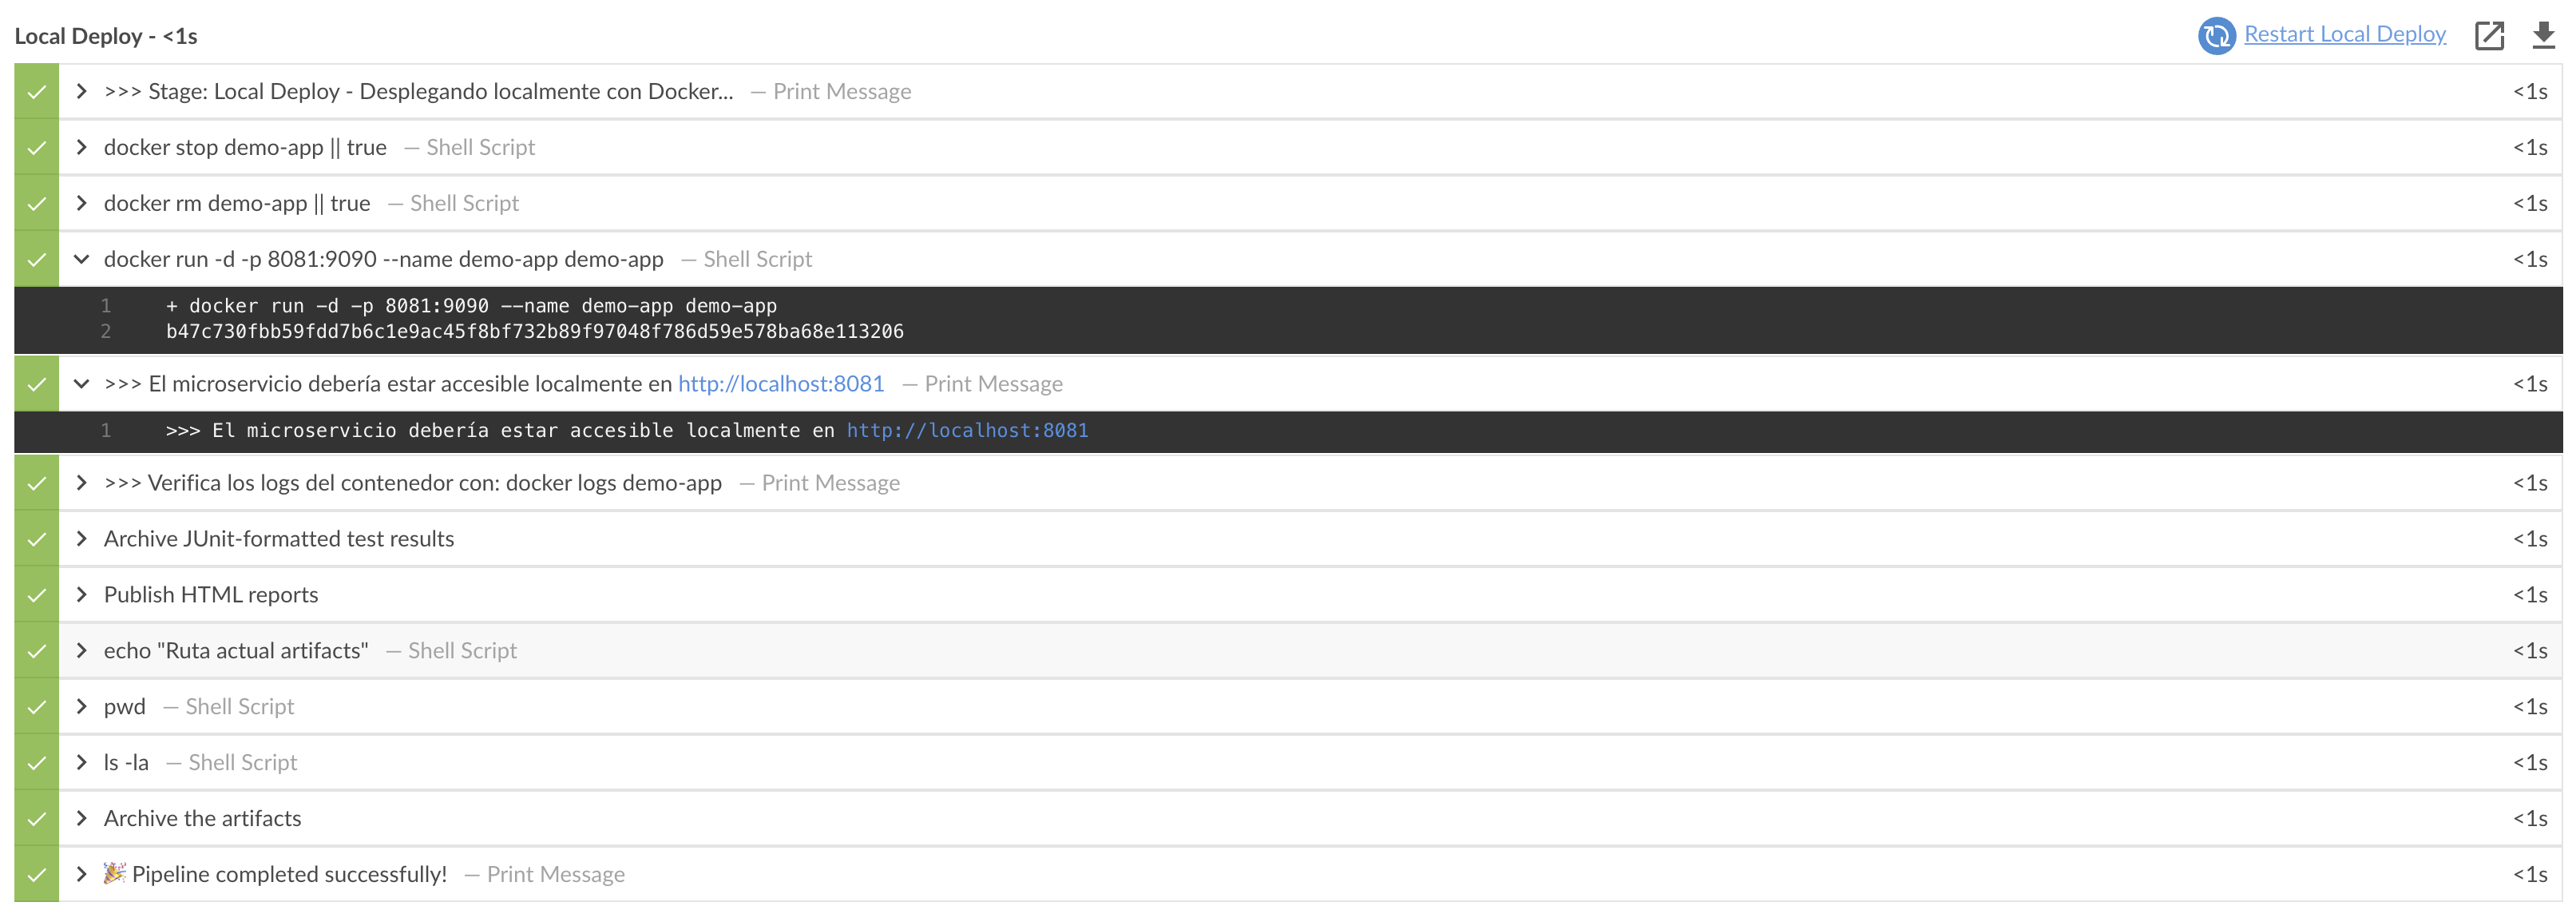
\includegraphics[width=0.9\textwidth]{contenido/imagenes/4_deploy_ok.png}
    \caption{Despliegue exitoso de la etapa de despliegue.}
    \label{fig:deploy_exitoso}
\end{figure}

En conclusión, el ciclo de evaluación demostró ser un éxito completo. La primera ejecución validó la capacidad del sistema para detectar riesgos y actuar como un mecanismo de control preventivo, deteniendo un despliegue inseguro. La segunda ejecución, tras aplicar las correcciones sugeridas por la IA, validó la utilidad y precisión de dichas sugerencias, permitiendo que un artefacto seguro completara el pipeline de principio a fin, como se evidencia en la ejecución final de la \textbf{Figura \ref{fig:pipeline_exitoso}}. Este proceso empírico confirma que la integración de asistencia por IA en un pipeline CI/CD no solo es viable, sino que acelera eficazmente el ciclo de remediación, cumpliendo así con los objetivos centrales de esta tesis.

\begin{figure}[H] 
    \centering
    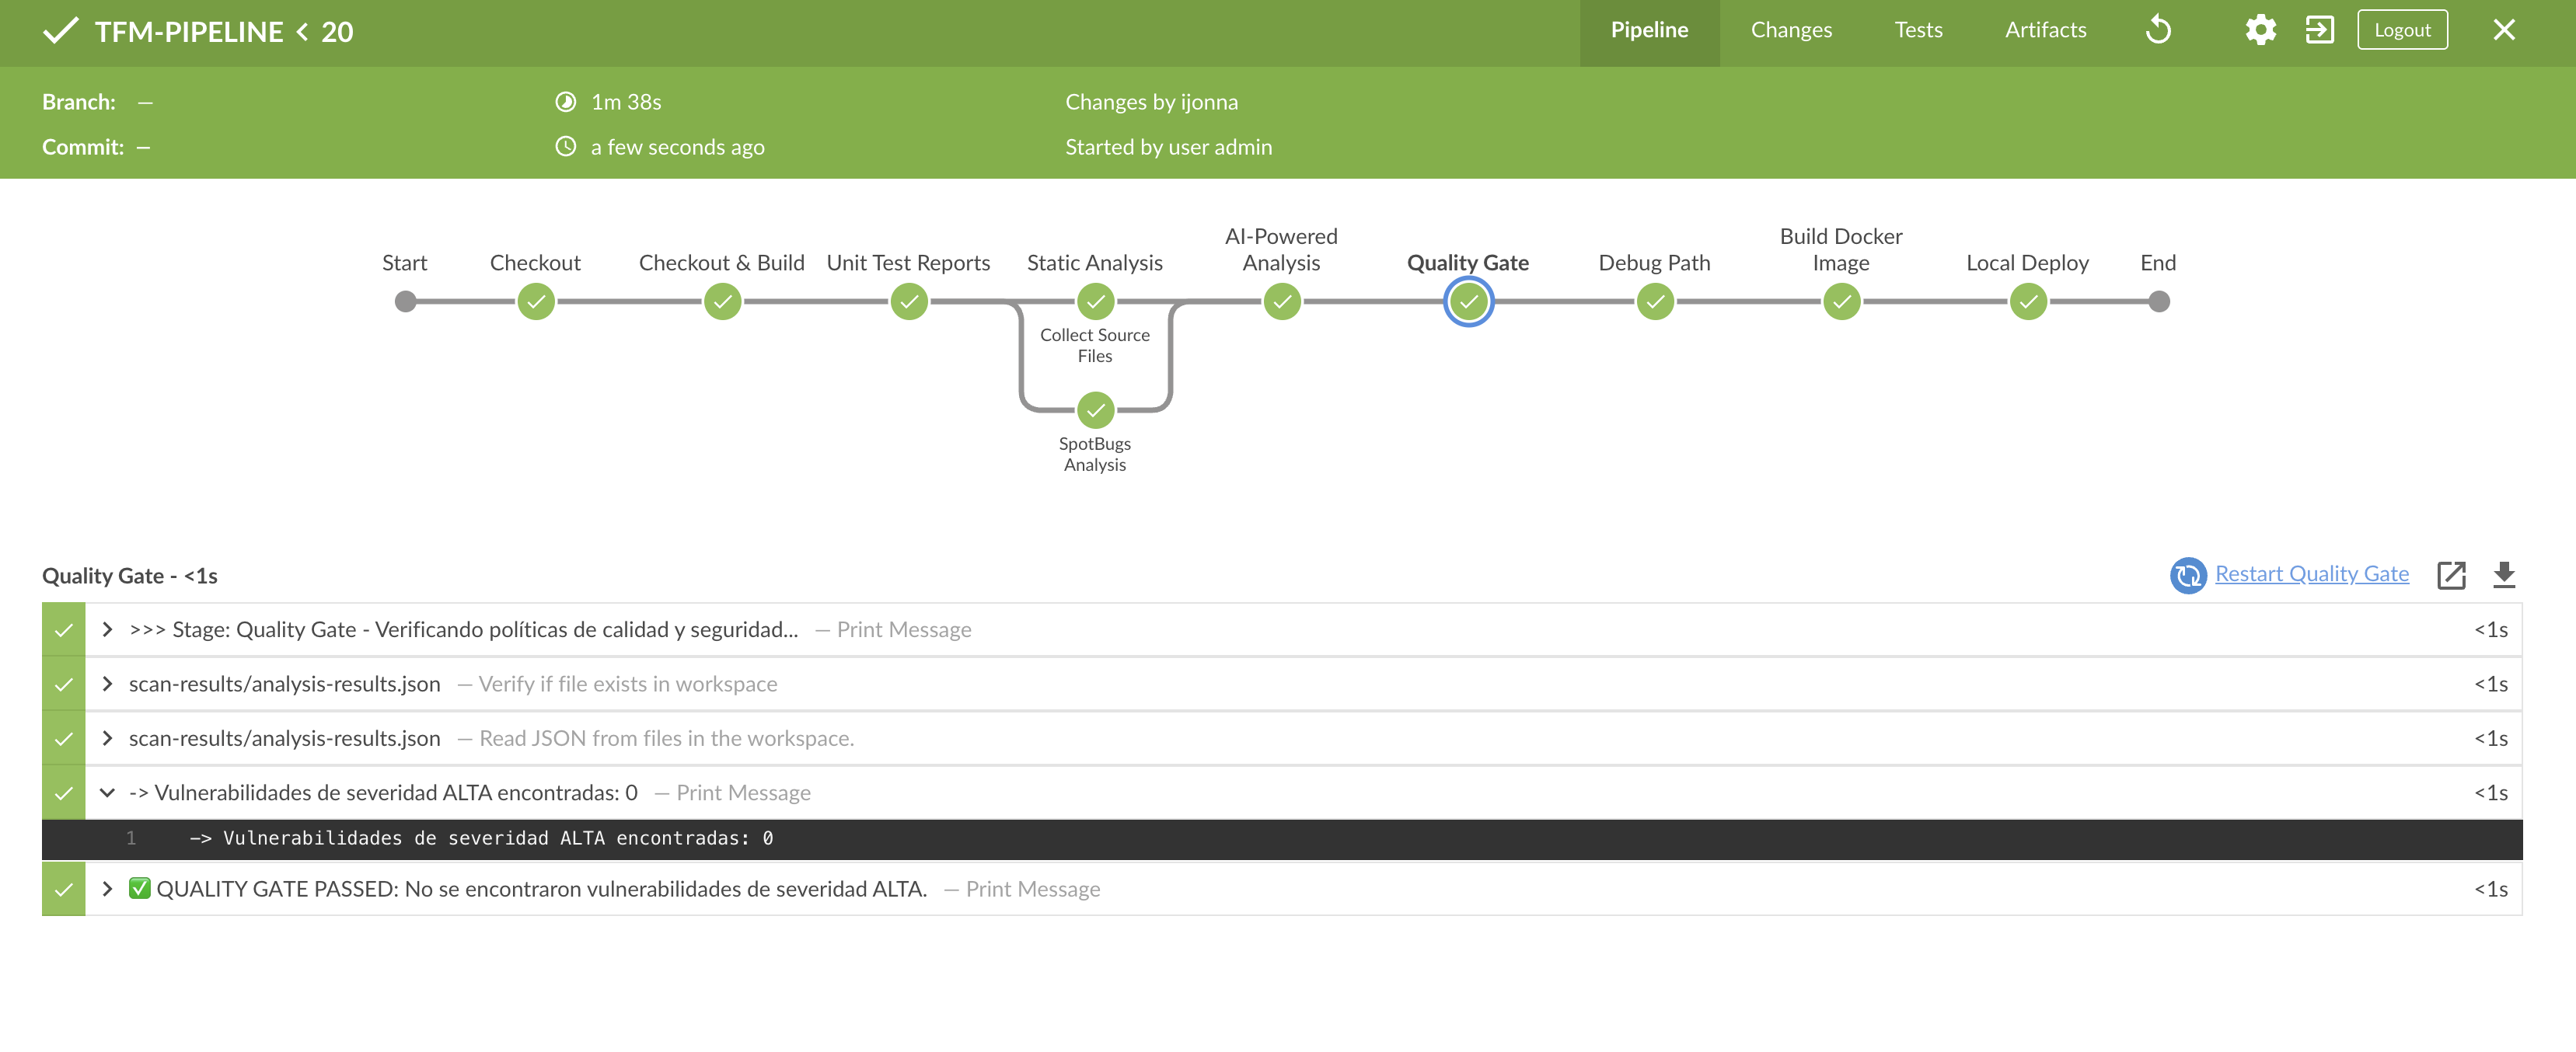
\includegraphics[width=0.9\textwidth]{contenido/imagenes/4_pipeline_ok.png}
    \caption{Ejecución exitosa del pipeline.}
    \label{fig:pipeline_exitoso}
\end{figure}

%%%%%%%%%%%%%%%%%%%%%%%%%%%%%%%%%%%%%%%%%%%%%%%%%%%%%%%%%%%%%%%%%%%%%%%
% FIN DEL CAPÍTULO 5
%%%%%%%%%%%%%%%%%%%%%%%%%%%%%%%%%%%%%%%%%%%%%%%%%%%%%%%%%%%%%%%%%%%%%%%